
\subsection{Answers}
\begin{table}[htb]%
\begin{center}%
\caption{Q23: Is there any room for performance tuning in your MPI programs? Select most suitable one.}%
\label{tab:Q23-ans}%
\begin{tabular}{l|l|r}%
\hline%
Choice & Abbrv. & \# Answers \\%
\hline%
{\small Yes, I know there is room for tuning but$\cdots$} & No resource & 317 (38.1\%) \\%
{\small Yes, I know there is room for tuning but$\cdots$} & Hard to rewrite & 153 (18.4\%) \\%
{\small I think there is room but I do not know $\cdots$} & No idea to tune & 104 (12.5\%) \\%
No, my MPI programs are well-tuned. & Well-tuned & 79 (9.5\%) \\%
{\small I do not know if there is room for perfo$\cdots$} & No idea to improve & 50 (6.0\%) \\%
I have no chance to investigate. & No chance to investigate & 48 (5.8\%) \\%
{\small I do not have (know) tools to find perfo$\cdots$} & Not having the tools & 29 (3.5\%) \\%
I do not know how to find bottlenecks. & No idea to find bottlenecks & 18 (2.2\%) \\%
other & - & 35 (4.2\%) \\%
\hline%
\multicolumn{2}{c}{total} & 833 \\%
\hline%
\end{tabular}%
\end{center}%
\end{table}%


\subsection{List of other answers}
\begin{itemize}
\item Europe:France: My job is to tune them
\item Europe:France: There is room but it's hardware dependant
\item Europe:France: Yes there remains room but the code will became too complex.
\item Europe:Germany: My programs are usually micro-benchmarks which evaluate performance of MPI.
\item Europe:Germany: Several communication patterns for adapting to implementation of MPI on a specific machine
\item Europe:Germany: There is overhead analysis to be done (tools programming).
\item Europe:Germany: Yes, I know there is room for tuning but re-writing the applications for performance must be balanced with other considerations.
\item Europe:Germany: Yes, based on regular benchmarking other people in my team do the tuning.
\item Europe:Germany: Yes, but first the algorithm has to work!
\item Europe:Germany: Yes, there is room, but the time consuming parts are already optimised
\item Europe:Germany: it depends, I have many projects
\item Europe:Italy: Yes, we plan to tune performance periodically
\item Europe:Italy: yes, to tune programs is my job
\item Europe:UK: I am actively working on it.
\item Europe:UK: I think there is room for tuning, but other developers are looking at it.
\item Europe:UK: Yes but "premature optimisation is the root of all evil" - i.e. it's good enough so better investing time elsewhere
\item Europe:UK: Yes, and am constantly doing so as the code evolves (\verb!>!100 devs)
\item Europe:UK: Yes, but I can not be bothered
\item Europe:UK: Yes, there is room for improvement. Justifying the developer time for the improvement can be challenging if the current performance is "good enough".
\item Europe:UK: Yes, we are doing this.
\item Europe:others: I think the MPI implementation could be tuned, but I had no time to experiment with that so far.
\item Europe:others: I work on MPI performance, but one can always do better.
\item Europe:others: No, the performance-critical layer is primarily OpenMP.
\item Europe:others: The application is latency bound, so even measuring at scale where a problem might exist is so hard it means we tackle other projects
\item Europe:others: There is always room for more tuning
\item Europe:others: Tuning employed when economically viable.
\item Europe:others: Yes and we are working on that
\item Europe:others: Yes, we are working on it.
\item Europe:others: most happens within PETSc, which is a well-tuned MPI library (I think)
\item Japan: Yes, but it's an MPI implementation issue.
\item Russia: My program - is MPI tool.So I do not need MPI performance tuning.
\item South Korea: Application performance varies according to the combination of MPI functions, so it is highly required to select apropriate ones.
\item USA: I believe there should be another option: "MPI does not provide the option that I need for performance tuning."
\item USA: Work on tuning is underway.
\item USA: Yes, I am actively doing tuning work

\end{itemize}

Only a very small fraction of the respondents (Les than 10\%) think that there
is no room for performance tuning of there application. However finding how to
optimize their MPI application is seen by the developers as a difficult
endeavor that requires too many resources (38.1\% of the answers), rewrite the
program (18\%). Interestingly more than 12\% of the respondent do not know how to
address performance issues of their program.  

\begin{figure}[htb]
\begin{center}
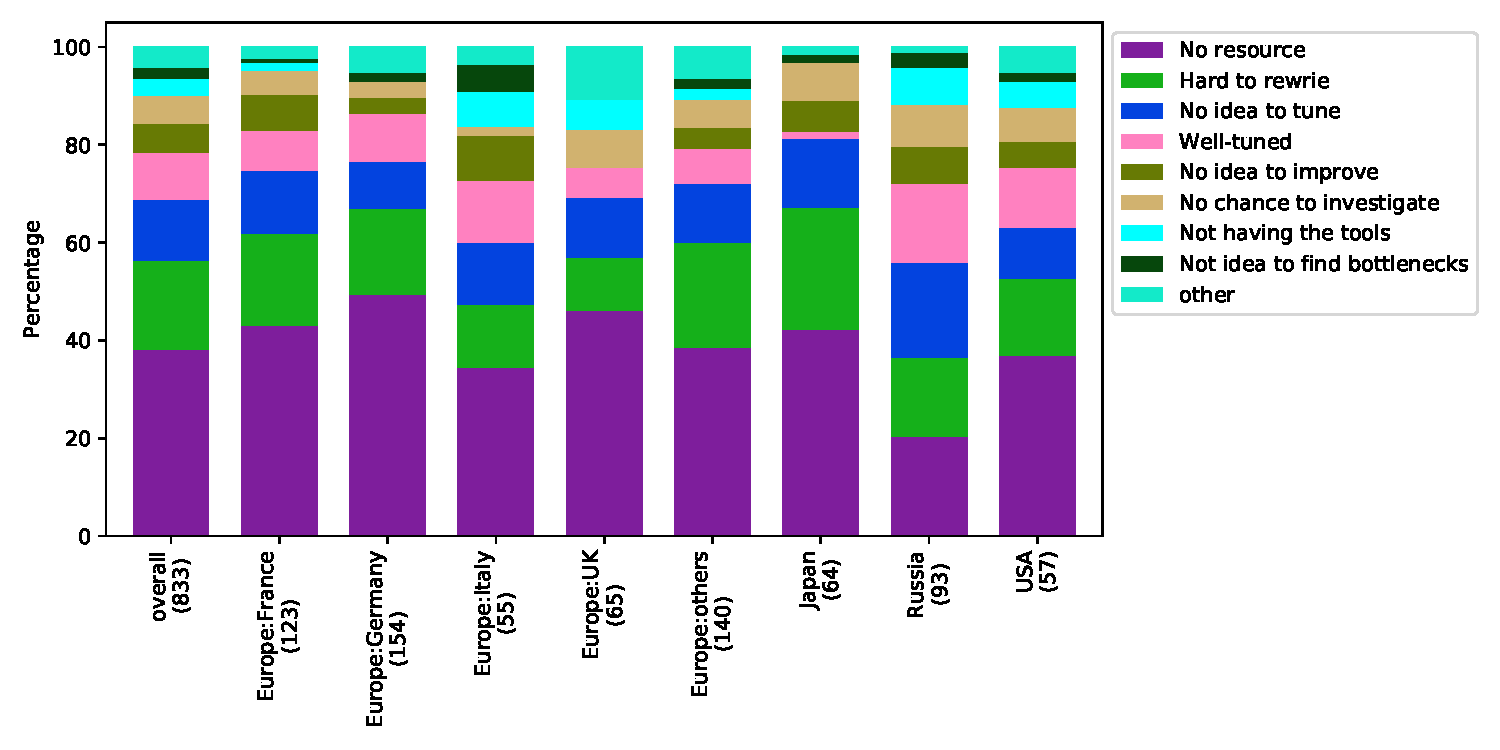
\includegraphics[width=10cm]{../pdfs/Q23.pdf}
\caption{Simple analysis: Q23}
\label{fig:Q23}
\end{center}
\end{figure}

Japan has the smalles percentage of the answer 'not tuned.' Is this
coming from their modesty?
